\begin{figure*}[htbp]
\centerline{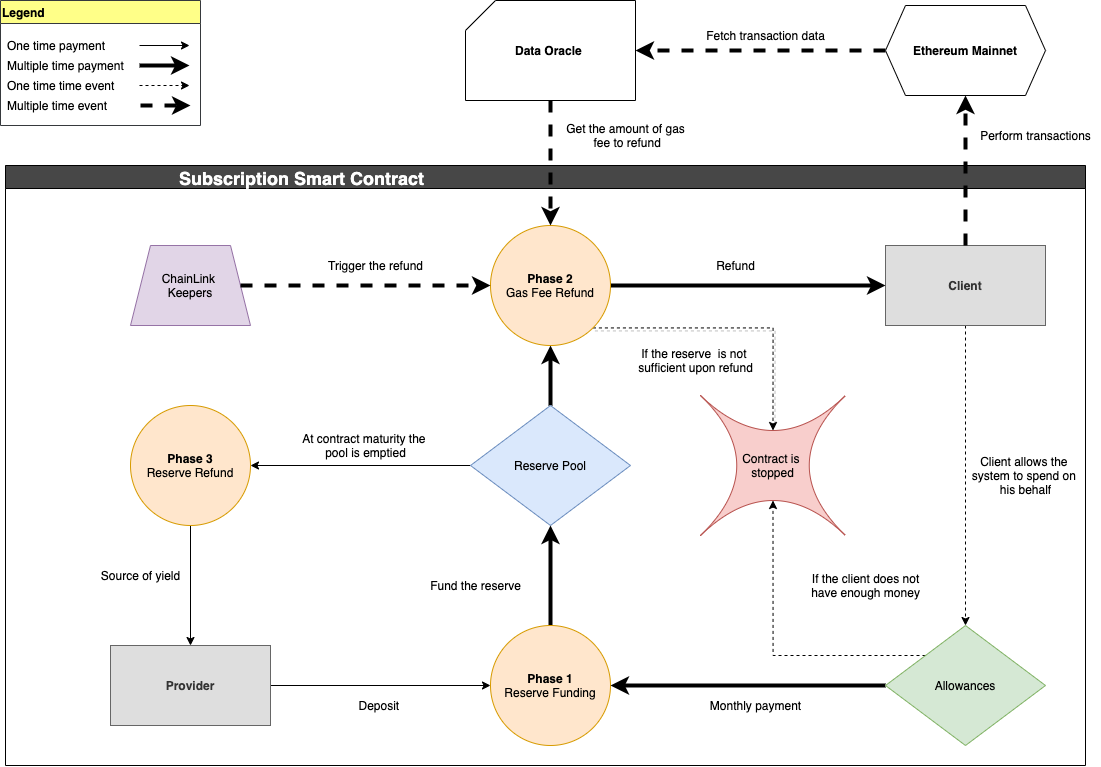
\includegraphics[scale=0.4]{figures/system-diagram.drawio.png}}
\caption{System dynamics}
\label{fig:system-diagram}
\end{figure*}

The intent of {\projectName} is to design a subscription system to tackle some of the problems induced by the volatility of gas fees on the Ethereum network. {\projectName} is decentralised and involves a subscription contract signed by the following main actors:
\begin{enumerate}
    \item A \textbf{client} for whom gas fees volatility is perceived as a valid reason to reduce its trading volume. He is willing to overpay for a system that provides him with reliable gas fees management. {\projectName} allows him to pay a regular and fixed amount of ETH to a provider to get his gas fees reimbursed and therefore hedge his risk.
    \item A \textbf{provider} who is assumed to have a good understanding of the blockchain infrastructure, markets and gas fees. Through the system, he locks some funds in a pool (used for future reimbursement of gas fees from the client) and speculates on a future low price of gas fees to generate yield. This yield is a bet on the fact that the amount generated by the regular payments made by the client is higher than the actual client gas fees consumption during the lifetime of the smart contract.
\end{enumerate}
Decentralisation, on top of anonymity guarantees for both providers and clients, motivates the choice of blockchain as the proper support of this system. 

An important consideration for the development of the system is the user-friendliness of the client intervention on the system. {\projectName} aims to make it as easy and automated as possible for the client to get his fees reimbursed.

A {\projectName} subscription contract between a provider and a client is defined in the terms of the variables shown in table \ref{tab:variables}. This contract operates by phases of $f$ blocks, defining a notion of time $t$ for the system. The dynamics of the system are described in detail in the following sections. They are also summarised in figure \ref{fig:system-diagram}.


\begin{table*}[htbp]
\caption{Smart contract variables}
\begin{center}
\begin{tabular}{|l|c|p{10cm}|c|}
\hline
\textbf{Name} & Ref.&  \textbf{\textit{Description}} & Unit \\
\hline
Maturity & $M$ & The time horizon of subscription. $M$ needs to be a multiple of $f$ & \# blocks. \\
Payment frequency & $f$ & frequency of the payments that the client has to do & \# blocks.\\
Payment amount & $x$ & the payment amount that shall be paid by the client, at frequency $f$. & ETH.\\
Initial reserve & $r$ & the amount of ETH that ht provider has to lock in the contract. This reserve is used to reimburse the client's transaction gas fees. & ETH. \\
Client's usage address  & $u_{add}$ & address registered by the client. The transaction performed by this address will be reimbursed. & ETH addr. \\
Client reimbursement address & $r_{add}$ & Address provided by the client where to send the reimbursement of transaction gas fees generated by $u_{add}$. & ETH addr.\\
Max operations & $n_{ops}$ & Dictionary that maps every kind of operation ("transfer","approve","swap"...) to an integer: the maximum number corresponding operations that can be refunded every $f$ blocks. & dictionary \\

Mean factor & $\alpha$ & upper bound on the reimbursement. The system only reimburses up to $\alpha$ times the current average  (over $k$ blocks) of the corresponding operation's gas fees. & float\\
\hline
\end{tabular}
\label{tab:variables}
\end{center}
\end{table*}

\subsection{Reserve Pool}
At the core of the system, there is a reserve pool from which ETH \footnote{As defined in section \ref{section:tokenomics}, the pool can also hold \$REF tokens} can be withdrawn to reimburse gas fees spent by the client in his personal external transactions. The pool is funded by two sources: 
\begin{enumerate}
    \item At the contract creation time ($t=0$), the provider needs to lock an initial reserve $r$ to provide default liquidity to the system.
    \item At the beginning of each phase ($t = f \cdot k \; \forall_{k = 0,1,\ldots,M/f}$), the client needs to pay a fee to be able to use the system. Without loss of generality, to ease the comparison with standard off-chain subscription systems, $f$ is set to a monthly frequency in the remaining sections.
\end{enumerate}
The reserve pool serves the purpose of financing the necessary gas fees to run the code of the system. These gas fees are referred to as "internal" in the following sections.

Finally, at maturity ($t=M$), the pool is emptied and the residual value is refunded to the provider. It marks the completion of the smart contract.

\subsection{Client monthly payments}

After signing the subscription smart contract, the client is subject to pay a monthly fee to finance the system until the contract maturity. One could argue that the system could be simplified to force the client to make one single bulk payment at signature time. However, it would induce several limitations on the client-side:
\begin{enumerate}
    \item \label{point:client-payment:bulk} The client may not have the necessary amount of ETH for the bulk payment at signature time. Spreading the bulk payment over multiple periods provides flexibility to the client.
    \item \label{point:client-payment:exit} The client may want to exit his position before maturity to discharge his liabilities to the system. For instance, such a situation could occur if the client believes he made a bad deal upon signing the contract or if he thinks he won't be able to cope with the future payments. In this case, the client wishes to extract as much ETH as soon as possible out of the system. However, the bulk payment will only be partially refunded when he finds a buyer for the existing contract. The issue is limited if we use spread payments. Indeed, at time $t < M$ only $  x \cdot \ceil{t/f} $ ETH have entered the system. In section \ref{section:tokens}, we demonstrate how such an exit can be implemented.
\end{enumerate}

Furthermore, the {\projectName} subscription contract also makes it possible for users to create such a bulk payment scheme by setting $F = M$. In that sense, we provide a broader action space to the users of the system.

In terms of implementation, we could consider various ways for {\projectName} to collect the client payments:
\begin{enumerate}
    \item Manual payments: the client needs to manually make a transaction of $x$ to the subscription contract before the beginning of each new phase. If no payment is made, the execution of the smart contract is stopped. If this option is rather simple to implement and could act as a trigger event for the refund system (cf. section \ref{section:refund}), it suffers from important drawbacks: 
    \begin{enumerate}
        \item Not user-friendly: an automated collection of payments would require fewer interventions on the client-side.
        \item Less incentive for the provider: the client can stop paying and leave the system which does not benefit the provider.
    \end{enumerate}
    \item Private payment pool: an alternative to the manual payment is to ask the client to lock $x \cdot f$, the full amount he needs to pay throughout the contract lifetime, upon signature into a private pool (not used to repay gas fees). This pool will automatically trigger a payment to the main {\projectName} reserve pool at the beginning of each phase. Compared to the first approach, the pool play the role of insurance both for the system and the provider. We mention that this implementation has the same drawbacks as the bulk approach defined at the top of this section. However, since the pool is private to the client, its content cannot be used to pay internal gas fee. Therefore, it reduces the amount that can be lost if the client wants to exit at some point.
    \item Allowances: finally, we can make use of the ERC-20 allowances interface to make the client give his approval for {\projectName} to spend some ETH on his behalf. The allowance would be initially set to $x \cdot f$ and {\projectName} will collect $x$ at the beginning of each phase. Allowances are simple to use and easy to implement. However, given all scams tokens that have risen in the past few years, the Ethereum community requires security guarantees to trust {\projectName} code. Hence, auditing costs are expected to be higher for this type of implementation.
\end{enumerate}
Given the user-friendliness and flexibility constraints stated in this section, the allowances choice is a better fit for {\projectName}. 

\subsection{gas fees refund} \label{section:refund}

In {\projectName}, the client pays a fixed monthly fee $x$ that allows him to get refunded the gas fees spent for his personal transactions on the Ethereum Mainnet. 
To avoid abusive behaviour on the client-side, we need to restrict the refund power in the following two aspects:
\begin{enumerate}
    \item The maximum number of monthly transactions for which {\projectName} will refund the associated gas fees. For instance, if set to $100$, it only allows for $100$ refunded gas fees transactions. If this restriction didn't apply, the customer could always generate a large number of transactions to empty the reserve pool, resulting in a large loss for the provider. No provider would use the system in this situation. We generalise further this notion to any operation ($n_{ops}$) that can be performed (e.g. "transfer", "approve", "swap", etc.) in the Mainnet to better capture the differences in gas fees of this operations. $n_{ops}$ is therefore defined as a dictionary mapping events to integers. 
    \item An upper bound of the reimbursement per operation called the mean factor $\alpha$. Indeed, upon performing a transaction the client can choose how much gas to use. The more he uses, the faster the operation validation is. Without this restriction, a client would always choose very high gas fees with negatively impacts the provider incentives to use the system. Therefore, the smart contract will only reimburse gas fees up to $\alpha$ times the current average (over $k$ blocks) of the corresponding operation's gas fees. For example, if $\alpha=1.25$ and that the average gas price for a swap operation is currently $50Gwei$ then the client can use up to $50\cdot1.25=62.5\:Gwei$ for a swap.
\end{enumerate}

\subsubsection{Fetching client transactions data} \label{section:oracle}

To reimburse the client gas fee, the contract has to be aware of all his transactions. Thus, a transaction tracking mechanism for the address $u_{add}$ needs to be implemented. Since our system cannot be hosted in layer 1 (cf. section \ref{section:host-chains}), the project will operate on a different level than the transactions to be fetched. A data oracle\cite{ethereumfoundationDecentralizedOraclesReliably2018} is the solution to this problem.

Two options are available:

\begin{enumerate}
    \item Centralised: a server using the Etherscan API\cite{EtherscanAPIs}. Transactions of client $u_{add}$ are accessible at the web address "https://etherscan.io/address/$u_{add}$". Etherscan offers multiple plans for real-time APIs.
    \item Decentralised: a framework such as \textit{Graph}.
\end{enumerate}
At this early step of the system, the centralised solution was chosen, mostly to simplify the development process.

To improve security, we also need to decentralise the way the off-chain data is collected. To this end, \textit{Chainlink Off-Chain Reporting}\cite{ChainlinkAchievesMajor2021} will be used to build a network of nodes calling the API and aggregating the data on-chain.

\subsubsection{The refund procedure}

To facilitate the use of the system and increase user experience for the client, {\projectName} will fetch the client transactions,  and decide when a refund applies. In other words, the client does not have to register transactions manually to the system. The provider can also benefit from this because it forbids the user to only register transactions with high gas fees. 

For each transaction made by the client, there are three main components of the refund procedure:
\begin{enumerate}
    \item Perform: the client performs the transaction on the Mainnet without interacting with {\projectName}.
    \item Fetch data: the oracle defined in section \ref{section:oracle}, will fetch the data information and extract the number of gas fees paid. 
    \item Refund gas fees: using this information, a \textit{refund} function can be triggered in the smart contract receiving as input the gas fees amount from the data oracle.  
\end{enumerate}

As a side note, if upon receiving a refund request, the reserve pool is empty (or not sufficient to perform the full refund) the contract terminates and both the provider and client are released from their obligations.

In terms of implementation, this automatic mechanism is not trivial. Indeed, the system needs events to be able to trigger the chain of actions resulting in the actual refund for the client. If the user was required to manually register the transactions to the system,
this registration event could simply be used as a trigger. However, it is not an option in {\projectName} as previously discussed. 

A simple way to  overcome this issue would be to extend the data oracle server to periodically fetches data in an automated way. Each update event can be used to trigger the smart contract refund function. However, this implementation severely reduces the decentralisation and security benefits of the system. A loop needs to be run on the server which represents a single point of failure.

Recently, \textit{Chainlink} launched the \textit{Keepers}\cite{IntroductionChainlinkKeepers} project which exactly serves this automation purpose in a decentralised and reliable way. \textit{Chainlink Keepers} makes a decentralised network of nodes available that are rewarded to execute jobs based on predefined conditions (e.g. time).  

Making Keeper-compatible contracts\cite{MakingKeepercompatibleContracts} simply requires implementing two functions:
\begin{enumerate}
    \item \textit{performUpkeep}: a call to the {\projectName} \textit{refund} method.
    \item \textit{checkUpkeep}: condition checker. For {\projectName} it acts as a scheduler and multiple options can be considered:
    \begin{enumerate}
        \item New transaction event: each time \textit{checkUpkeep} is called, the data oracle is called as well. If the latter returns new gas fees to be refunded for some users, then the condition status is set to true. In other words, with this method, gas fees are refunded soon after the transaction is confirmed in the Mainnet which provides flexibility for the client. However, due to the complexity of the implementation and the frequency of checks, higher internal gas fees consumption is to be expected compared to point \ref{point:monthly-refund}. 
        \item \label{point:monthly-refund} End of month event: in this case, \textit{checkUpKeep} simply check that the current block number corresponds to the end of the monthly period. It is equivalent to make one bulk payment to refund all gas fees spent in the client's last month utilisation. It is cheap in terms of internal gas fees consumption but lacks flexibility since the client needs to wait until the end of the period to get the refund.  
    \end{enumerate}
\end{enumerate}

Eventually, {\projectName} will support both types of \textit{checkUpkeep} functions to provide higher flexibility to the users of the system.


\subsection{Host chains} \label{section:host-chains}
Implementing the project on the Ethereum layer 1 itself is not a good solution because using the contract might also involve high gas fees upon running. Indeed, the system achieves nothing if the process of reimbursing a single transaction cost more gas fees than the transaction itself. 

Scaling \projectName to layer 2 allows the contract to operate within the layer, achieving both lower fees, while still ensuring communication and compatibility with the first layer to track the client's transaction.

In terms of blockchain infrastructure, {\projectName} will first be hosted on \textit{Polygon} to leverage the power of layer 2 and \textit{Chainlink Keepers}. In the future, if more networks are supported by the \textit{Chainlink Keepers} project, we may consider hosting {\projectName}  on several other layer 2 solutions to increase availability for users.

% Describe which substructure to use in Polygon.

\subsection{{\projectName} Tokens and Smart Contracts} \label{section:tokens}

In this section, we aim to demonstrate how {\projectName} can be modelled as a set of smart contracts, operating between the provider, the client and the oracle. For reasons that will be explained in the following paragraphs, we chose to model {\projectName} using the following building blocks: 
\begin{enumerate}
    \item A native token  \$REF 
\end{enumerate}



To conclude the system will support the following list of requirements: 
\begin{enumerate}
    \item The subscription contract can be created by either the provider or the client. 
    \item Only one party needs to be specified upon creation. 
    \item The party responsible for the creation can trade ownership on the contract via a NFT marketplace.
    \item In the NFT marketplace, contract prices are set by the levels of the demand and the offer.  
    \item The creation phase amounts to fill in the variables highlighted in table \ref{tab:variables}. 
    \item Any party can decide to resell his ownership token on the NFT marketplace. If the token is bought, the new owner shall respect the contractual obligations defined at contract creation time.
\end{enumerate}

In practice, at contract creation time, both provider and client addresses are set to the creator address. Then, the creator can trade/give the ownership of one side of the contract on a NFT marketplace. For example, if the creator wants to be the provider of the subscription, he will trade the client-side token. The buyer of the token then becomes the client. 

The contract starts whenever the two addresses (client and provider) are different. During the subscription lifetime, we provide flexibility by allowing any party can trade its ownership token and exit the system. When ownership is traded, the contract simply updates the concerned address. The easiest way to implement this mechanism would be to only use the native token of the system (\$REF) for the trades. In that case, all transactions would be internal to the {\projectName} system and could be implemented by keeping track of users' balances and using transfer functions. But ownerships could also be traded as NFTs (ERC-721) on different marketplaces (ex: \href{opensea}{https://opensea.io/}). In that case, a user can claim one ownership using a "claim" method of the contract. This method checks if the claimer processes the corresponding NFT and updates one of the addresses if yes.

Having the possibility to trade ownerships allows the actors to easily (assuming liquidity is high) get rid of theirs position. Imagine the scenario where a provider locks some funds in a subscription contract and some days later realizes that the Gas price will go up. This provider can then sell his ownership to someone else and avoid losses. Trading ownerships also allows the client to speculate on the gas price going up. Imagine a client starts a contract with a long maturity when the gas price is low, then if the gas prices suddenly rise the client can sell his ownership to another client for a higher price than the initial and make some profit.
More information on the tokenomics of the system can be found in section \ref{section:tokenomics}.


\subsection{Tokenomics} \label{section:tokenomics}

{\projectName} system is ruled by the \$REF a governance token. This token acts as voting power and can be used to trade contracts. \$REF follows the ERC-20 standard. 

Holding some of the native tokens (\$REF) involves multiple benefits: 
\begin{enumerate}
    \item The system's DAO relies on the native token \$REF. Having \$REF tokens allows the owner to vote on the future of the project.
    \item Whenever a contract terminates, a small part of the final reserve pool is evenly distributed to the token holders. This reward is paid in ETH or \$REF, depending on the token used by the contract. 
    \item As explained in section \ref{section:tokens}, the ownership of a contract (client or provider side) is tradable and again every time such a transaction happens, a small part of the established price is redistributed to token holders. 
\end{enumerate}

{\projectName}'s subscription contract will allow users to agree on the currency used by the system. Users will be able to choose between ETH and the {\projectName} native token (\$REF). Specifically, all transactions made to the pool and refunded gas fees will occur in the specified token. To attract people on using the \$REF token, a premium is distributed to both parties of a subscription contract, in \$REF, that terminates. In that case, since the unit of gas fees is GWEI (ETH), we need to incorporate a swapping mechanism between ETH and \$REF. A possible implementation would be to use Uniswap with some default base rate. The actual details of such a mechanism are left for further study.


\subsubsection{The {\projectName} decentralised application}

To increase user experience, the {\projectName} system will be powered up by a decentralised application. Its purpose is threefold:
\begin{enumerate}
    \item A platform to create and deploy smart contracts on one of the supported layer 2 solutions. Two creation modes will be offered:
    \begin{enumerate}
        \item Basic: a simple approach with predefined smart contract variables for non-experienced users
        \item Professional: this mode leverages the full power and flexibility of the system by allowing any values of the smart contract variables.
    \end{enumerate}
    \item A NFT marketplace to trade the contract. 
    \item A personalised view for a user to display relevant information of his owned contracts (current yield for the provider, amount refunded for the client, etc.).
\end{enumerate}


